\documentclass[french]{article}
 
\usepackage[utf8]{inputenc}
\usepackage[T1]{fontenc}
\usepackage{babel}
\usepackage{graphicx}
\usepackage{amsmath}
\usepackage{caption}

\begin{document}
\section{Tension de surface}
\begin{figure}[ht]
	\centering
	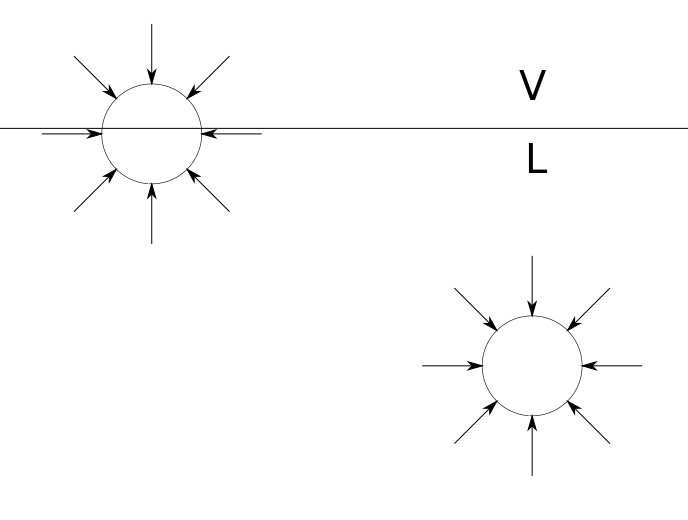
\includegraphics[scale = 0.3]{./image/rondforces.png}
	\caption{Ligne triple}
\end{figure}
La tension de surface est une force par unité de longueur.\\ 

Dans un liquide ayant une interface, une molécule complètement immergée dans le liquide est soumise à des forces d'interactions avec les autres molécules (du liquide) dans toutes les directions. 

Une molécule située à l'interface, la somme des interactions (avec les molécules du même fluide) est non nulle est dirigée vers l'intérieur du liquide. Il existe donc une force supplémentaire qui permet de maintenir l'interface.

Cette force supplémentaire (par unité de longueur) est la tension de surface.\\



la tension de surface est aussi une énergie par unité de surface, c'est l'énergie (par unité de surface) pour séparer les interfaces et les envoyer à l'infini.


\subsection{Mouillage}
Le mouillage est l'action de mouiller et mouiller consiste à  mettre en contact avec un liquide.
\begin{figure}[ht]
	\centering
	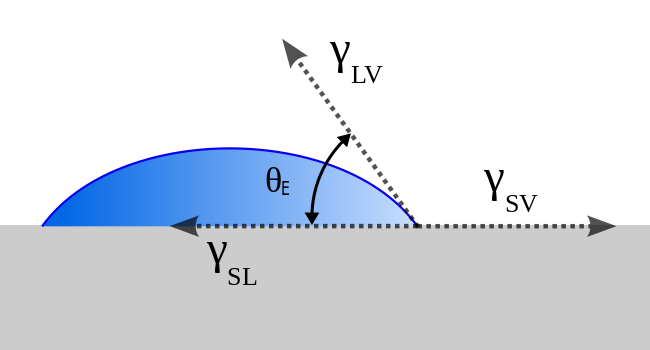
\includegraphics[scale = 0.3]{./image/Contact_angle2.png}
	\caption{Ligne triple}
\end{figure}

Nous nous intéressons en particulier au contact d'une goutte dont le support est une plaque plane. 


Le substrat est le nom donné au support (solide ou liquide) sur lequel la goutte de liquide repose.

Lorsqu'une goutte d'eau est posée sur support solide, il y a formation de 3 interfaces et donc de 3 tensions de surface.


En projetant les tensions de surface sur l'horizontale :

\begin{equation}
	\label{eq:Young}
	\gamma_{SV}  = \gamma_{SL} + \gamma_{LV}\cos\theta_{E}
\end{equation}

C'est la loi de Young.


Tout de même, en parcourant la littérature lors de l'écriture de notre rapport, nous avons pu constater que les auteurs n'étaient pas d'accord concernant $\gamma_{SV}$ en refusant de l'appeler tension de surfae.


Cela a été beaucoup destabilisant puisque $\gamma_{SV}$ est appleé tension de surface par plusieurs autres auteurs.

C'est l'article \textit{Young's equation revesited} publié dans \emph{Journal of Physics} le 4 Mars 2016 qui a répondu à nos intérrogations.


\newpage
\begin{figure}
\centering
\begin{minipage}[c]{\textwidth}
\centering
	\includegraphics[scale = 1]{./image/cmaa16e7f02_hr.jpg}
    \caption{Caption for image}
    \label{fig:sample_figure}
\end{minipage}
\end{figure}
\begin{equation}
	\label{eq:Young-revisted}
	\sigma_{s}  = \gamma_{SL} + \gamma_{LV}\cos\theta_{E}
\end{equation}

Où $\sigma_{s}$ est la compasante composante tangentielle du vecteur de la surface du solide autour du point où l'angle de $\theta_{E}$ est mesuré.
\begin{description}
\item[$S < 0$ :] Mouillage partiel
\item[$S > 0$ :] Mouillage total
\end{description}


Lorsque la goutte est en mouvement, l'angle dynamique   entre 2 liquides non miscibles ou entre un liquide et l'air ou en un liquide et une surface.

La tension de surface 

La capillarité étudie l'interface entre l'air et un liquide ou entre 2 liquides
non miscibles.

Le mouillage est l'action de mouiller et mouiller consiste à mettre en contact avec un liquide.

Nous nous intéressons en particulier au contact d'une goutte avec un support matériel.

C'est le paramètre d'étalement $S = \gamma_{SG} - \gamma_{SL} - \gamma_{LG}$ qui caractérise le mouillage lorsque la goutte est en équilibre sur un support matériel.

\begin{description}
\item[$S < 0$ :] Mouillage partiel
\item[$S > 0$ :] Mouillage total
\end{description}

Lorsque la que est en équilire nous avons:

\[\gamma_{SG}\ = \gamma_{SL} - \gamma_{LG}\cos\theta_{E} \]

\begin{figure}[ht]
	\centering
	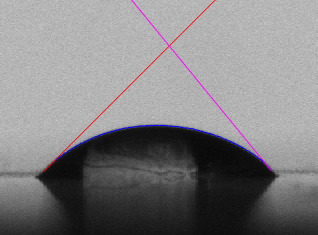
\includegraphics[scale = 0.6]{./image/crop_tvitesse=28_volume=003.png}
	\caption{Goutte d'eau de volume $0.03$ml avec $\theta_{a} = 45^{o}$ et $\theta_{r} = 50.17^{o}$}
\end{figure}

\begin{figure}[ht]
	\centering
	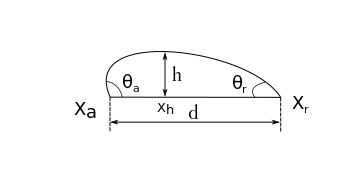
\includegraphics[scale = 0.6]{./image/rrgou.png}
	\caption{Goutte d'eau de volume $0.03$ml}
\end{figure}
\end{document}
